\documentclass[11pt]{article}

\usepackage[utf8]{inputenc}
\usepackage[T1]{fontenc}
\usepackage{lmodern}
\usepackage[margin=1in]{geometry}
\usepackage{microtype}
\usepackage{amsmath,amssymb,amsthm,mathtools}
\usepackage{booktabs}
\usepackage{multirow}
\usepackage{array}
\usepackage{graphicx}
\usepackage{xcolor}
\usepackage{hyperref}
\usepackage{url}
\usepackage{enumitem}
\usepackage{float}
\usepackage{caption}
\usepackage{subcaption}
\usepackage{ifthen}
\usepackage{longtable}
\usepackage{tabularx}
\usepackage{listings}
\usepackage{setspace}

\hypersetup{
  colorlinks=true,
  linkcolor=blue!60!black,
  citecolor=blue!60!black,
  urlcolor=blue!60!black
}

\title{\textbf{Replay Levels and Nondeterminism Detection for Agentic CPS}}
\author{Anonymous Authors}
\date{}

\newcommand{\tool}[1]{\texttt{#1}}
\newcommand{\field}[1]{\texttt{#1}}
\newcommand{\code}[1]{\texttt{#1}}
\newcommand{\Lzero}{\mathrm{L0}}
\newcommand{\Lone}{\mathrm{L1}}
\newcommand{\Ltwo}{\mathrm{L2}}
\newcommand{\trace}{\mathcal{T}}
\newcommand{\event}{e}
\newcommand{\state}{s}
\newcommand{\hashf}{H}

\newtheorem{definition}{Definition}
\newtheorem{proposition}{Proposition}
\newtheorem{assumption}{Assumption}

\begin{document}
\maketitle

\begin{abstract}
Replayability is a missing assurance primitive for agentic cyber-physical systems (CPS). Logs are insufficient for independent replay verification: they may record what happened, but not whether the same trace re-executes to the same control-plane state or where hidden divergence first appears. We present a replay framework organized into replay levels \Lzero/\Lone/\Ltwo, with a concrete, evaluated \Lzero{} contract for per-event verification and first-divergence localization. The goal is intentionally narrower than whole-process record/replay: we target independently checkable control-plane evidence under declared trace semantics, not full-process or hardware determinism. Traces carry sequence number, time, event type, actor, payload, and state-hash commitments; replay re-applies events, recomputes state, and emits structured diagnostics when replayed and committed hashes differ. We evaluate over explicit evidence lanes: synthetic traps, synthetic passes, field-proxy traces, and a real-ingest example. On the evaluated corpus, expected pass/fail outcomes are met and seq-labeled traps localize at the expected event. Replay outputs are integrated into evidence bundles for audit-style use. On the publishable run (20 replays of the primary thin-slice trace), full \Lzero{} replay has mean overhead 0.3495\,ms, empirical p95 0.6911\,ms, and empirical p99 0.7821\,ms; the paired full-vs-apply-only mean difference is 0.3251\,ms (95\% bootstrap CI [0.2613, 0.3989]\,ms). We do not claim fleet-scale determinism, hardware equivalence, or physics replay. The contribution is a contract-bounded CPS evidence path: replay levels, a CPS-aware trace contract, sequence-level nondeterminism localization, structured diagnostics, and bounded verification overhead against explicit baselines.
\end{abstract}

\section{Introduction}

Modern agentic CPS already produce extensive execution traces. Yet most traces remain observational artifacts rather than replay contracts. They support post hoc inspection, but often do not support independent third-party verification that the same trace re-executes to the same control-plane behavior, nor do they explain where a hidden nondeterministic divergence first appears. This matters for safety cases, audit, forensics, and reproducible evaluation. In these settings, ``we have logs'' is not the same as ``we have independently checkable replay evidence for control-plane claims.''

\paragraph{Motivating failure vignette.}
A laboratory workflow trace appears normal and a downstream run-completion report looks successful. During review, an auditor denies release because a gate-level decision and reported state commitments are inconsistent. Raw logs do not identify whether the discrepancy came from scheduling order, stale control-plane state, or silent nondeterminism. Under the \Lzero{} replay contract, the first violating event is localized (with expected-vs-observed hash and witness context), and the resulting diagnostic is exported into the evidence bundle. This turns ambiguity into an auditable, machine-checkable failure record.

This paper addresses that gap. Our goal is not full-process record/replay, instruction-level determinism, or hardware-faithful re-execution. Those are important but distinct problems. Instead, we ask a focused systems question: \emph{what is the smallest replay contract that still yields independently checkable CPS evidence?} Our answer is a replay framework with explicit replay levels and a concrete \Lzero{} contract. At \Lzero{}, replay re-applies the trace in deterministic sequence order, recomputes control-plane state, checks per-event state hashes, and emits structured diagnostics on divergence. The primary guarantee is therefore not ``perfect fidelity of everything,'' but \emph{detection and localization of control-plane divergence relative to a declared replay contract.}

That scope discipline is important. Many real CPS deployments do not need or cannot afford whole-process replay. What they need is something more modest and often more actionable: independent verification that the traced control plane is consistent with a declared semantics, and a witness of the first event at which it is not. That witness can then enter an evidence bundle, support conformance checks, or drive forensic triage.

\paragraph{Scientific question and testable predictions.}
We evaluate a single scientific question: under a declared control-plane replay contract, can replay produce independently checkable evidence with localizable first divergence at acceptable incremental cost? The paper tests this with three measurable predictions: (i) seq-labeled trap traces localize at expected divergence positions, (ii) corpus outcomes satisfy expected pass/fail behavior across evidence lanes, and (iii) full \Lzero{} adds bounded overhead relative to weaker baselines.

Our contributions are:

\begin{enumerate}[leftmargin=1.5em]
    \item A replay model for agentic CPS organized into replay levels \Lzero{}, \Lone{}, and \Ltwo{}, with \Lzero{} fully implemented, \Lone{} partially implemented as a control-plane twin contract, and \Ltwo{} defined only as design scope in this version.
    \item A CPS-aware trace contract in which events carry enough control-plane structure --- including \field{seq}, \field{ts}, \field{type}, \field{actor}, \field{payload}, and \field{state\_hash\_after} --- to support third-party \Lzero{} replay and per-event verification.
    \item A replay engine and divergence detector that localize the first mismatching sequence position and emit structured diagnostics including expected hash, observed hash, event type, and witness context.
    \item An evaluation over a replay corpus and overhead benchmarks showing that the implementation meets expected pass/fail outcomes on the corpus, localizes trap divergences at the expected sequence, and incurs bounded sub-millisecond overhead on the primary thin-slice trace.
\end{enumerate}

\section{Scope and positioning}

The paper is intentionally narrow in three ways.

First, the replay target is the \emph{control plane}, not the whole process. We do not attempt instruction-by-instruction replay, kernel capture, device timing reproduction, or hardware determinism. Second, the primary deliverable is \emph{detection and localization}, not rollback or recovery. Third, the evaluation is over thin-slice traces, traps, and a field-style proxy trace, not over a production fleet.

This deliberate scoping differentiates the paper from at least three adjacent categories. It is not a whole-process record/replay system such as RR-style debugging infrastructure. It is not merely a log viewer, because it checks per-event state commitments and localizes divergence. And it is not a full physics twin, because \Lone{} in this paper remains a control-plane replay level with recorded observations rather than a simulator-backed world model.

We frame this as a design choice, not a concession: when the assurance target is control-plane evidence, whole-process replay is often the wrong abstraction because it is costlier, harder to deploy, and unnecessary for the claim being verified.

\section{Related work}

\paragraph{Record/replay and deterministic debugging.}
Record/replay systems have long demonstrated the value of reconstructing executions for debugging and forensics. ReVirt moved logging below the guest operating system to enable replay for intrusion analysis \cite{dunlap2002revirt}. RR emphasized deployable user-space record/replay for debugging complex software with modest overhead \cite{ocallahan2017rr}. These systems target much stronger replay guarantees than we do. Our work differs in both ambition and artifact surface: we do not seek whole-process determinism, kernel-level replay, or instruction-level debugging. Instead, we target control-plane replay over a structured CPS trace, with explicit state-hash commitments and sequence-level localization of divergence.

\paragraph{Accountability and replay-based verification.}
PeerReview showed that signed logs and deterministic replay can support practical accountability in distributed systems \cite{haeberlen2007peerreview}. That work is particularly relevant because it treats replay as evidence rather than merely as a developer convenience. Our paper is closer in spirit to accountability than to debugger engineering. However, our scope is narrower: we work with a CPS-specific replay contract over a trace format, not with a general secure-log accountability framework across administrative domains.

\paragraph{CPS trustworthiness and evidence.}
The NIST CPS Framework emphasizes coordinated treatment of timing, data, trustworthiness, and interoperability rather than isolated mechanisms \cite{nist2017cps}. Our replay design follows that philosophy. Replay is not presented as a debugging add-on but as part of an evidence path: replay outcomes enter evidence bundles and can be consumed by higher-level assurance logic. This is why we make the trace semantics explicit and why replay levels are defined as contracts, not just modes of execution.

\paragraph{Provenance and workflow evidence.}
Standards for provenance interchange (e.g., W3C PROV \cite{w3c2013prov}) describe how to document entities, activities, and agents for reproducibility and audit. Our contribution is not a general provenance graph for arbitrary workflows; it is a \emph{control-plane} replay primitive that produces machine-checkable hashes and sequence-indexed diagnostics. When bundles are emitted in schema-compatible form, replay outcomes can align with broader provenance or assurance tooling, but the replay contract is intentionally narrower than full provenance capture.

\paragraph{Positioning.}
The novelty of this paper is not ``another replay tool.'' It is the combination of (i) explicit replay levels with bounded claims, (ii) a CPS-aware trace contract with per-event state commitments, (iii) sequence-level nondeterminism localization, and (iv) integration of replay outcomes into evidence bundles for audit-style use.

\paragraph{What is new here.}
The contribution is architectural and evidentiary: architectural because replay is tiered and contract-bounded; evidentiary because outcomes are exported as machine-checkable assurance artifacts. Concretely, this paper is not full record/replay, not secure-log accountability alone, and not a digital twin; it is the joint design of replay levels, CPS trace commitments, first-divergence localization, and evidence-bundle integration.

\begin{table}[H]
\centering
\caption{Contribution split between architectural and evaluation novelty.}
\label{tab:novelty-split}
\begin{tabular}{p{5.8cm}p{8.4cm}}
\toprule
Architectural novelty & Evaluation novelty \\
\midrule
Tiered replay contract (\Lzero/\Lone/\Ltwo) with explicit bounded claims; control-plane trace commitments coupled to first-divergence diagnostics; replay outputs mapped to assurance bundles. & Lane-separated corpus reporting (synthetic trap/pass, field proxy, real ingest), denominator-explicit localization accounting, baseline deltas quantifying the cost of admissible evidence, and supplementary multi-seed L1 twin summary. \\
\bottomrule
\end{tabular}
\end{table}

\section{Replay model}

\subsection{Worked example (intuition before formalism)}
Consider a short trace where events \texttt{0}--\texttt{2} apply cleanly: recomputed \field{state\_hash\_after} matches the trace at each step. At \texttt{seq=3}, recomputation yields $\hat{h}_3 \neq h_3$ while earlier hashes agree. Then $i^\star=3$: the first contract violation is at event 3, not at a later gate or report. Witness context (neighboring events and payloads) is attached to the diagnostic; downstream events may still run, but they are not needed to \emph{establish} the first mismatch. This is the operational content of first-divergence localization.

\subsection{Replay levels}

We define replay in three levels.

\begin{itemize}[leftmargin=1.5em]
    \item \textbf{\Lzero{} (implemented).} Control-plane replay from trace. Events are applied in declared order, control-plane state is recomputed, and replayed state hashes are compared against the trace. Divergence is detected and localized.
    \item \textbf{\Lone{} (partially implemented).} \Lzero{} plus replay against a declared twin configuration and recorded observations. In this version, \Lone{} is still a control-plane replay contract; it is not a physics replay claim.
    \item \textbf{\Ltwo{} (design only).} Hardware-assisted or hardware-coupled replay. \Ltwo{} is explicitly out of scope for this paper.
\end{itemize}

This level structure prevents a familiar overclaim in replay papers: treating a useful control-plane replay mechanism as if it were full determinism. It is not.

\subsection{Trace contract}

A trace is a finite sequence
\[
\trace = (\event_1, \event_2, \ldots, \event_n),
\]
where each event contains at least:
\[
\event_i = (\texttt{seq}_i, \texttt{ts}_i, \texttt{type}_i, \texttt{actor}_i, \texttt{payload}_i, h_i).
\]
Here $h_i$ denotes \field{state\_hash\_after}, i.e., the committed hash of the control-plane state after applying event $\event_i$ under the declared trace semantics.

\begin{table}[H]
\centering
\caption{Notation used in the replay model (formal section).}
\label{tab:notation}
\begin{tabular}{ll}
\toprule
Symbol / field & Meaning \\
\midrule
$\texttt{seq}_i$ & Event sequence index (trace may be 0-based; model index $i$ is 1-based) \\
$h_i$ & Committed post-event control-plane state hash from the trace \\
$\hat{h}_i$ & Recomputed post-event control-plane state hash during replay \\
$i^\star$ & First divergence index where $\hat{h}_i \neq h_i$ \\
\field{witness\_slice} & Local event context around $i^\star$ for diagnostics \\
\field{witness\_window} & Configured neighborhood width used to build witness slices \\
\bottomrule
\end{tabular}
\end{table}

Let $F$ denote the deterministic control-plane transition function. Starting from initial state $\state_0$, replay defines
\[
\state_i' = F(\state_{i-1}', \event_i), \qquad \hat{h}_i = \hashf(\state_i').
\]

\begin{definition}[\Lzero{} replay success]
An \Lzero{} replay of trace $\trace$ succeeds iff $\hat{h}_i = h_i$ for all $i \in \{1,\dots,n\}$ and the final state hash also matches the final committed state.
\end{definition}

\begin{definition}[First divergence]
If replay does not succeed, the first divergence position is
\[
i^\star = \min\{ i : \hat{h}_i \neq h_i\}.
\]
The replay engine emits diagnostics that include at least $i^\star$, the expected hash $h_{i^\star}$, the observed hash $\hat{h}_{i^\star}$, and the corresponding event context.
\end{definition}

\begin{assumption}[Deterministic transition semantics]
For the evaluated \Lzero{} contract, the replay transition function $F$ is deterministic over the declared event ontology and payload semantics.
\end{assumption}

\begin{assumption}[Practical collision resistance in-scope]
State commitments are treated as collision-resistant for the evaluated traces; no collision is observed in the corpus, so hash mismatch is interpreted as state mismatch for this scope.
\end{assumption}

\begin{assumption}[Ingestion integrity outside replay core]
Trace authenticity/integrity at ingest is a separate systems concern. The replay checker assumes provided trace bytes are the intended artifact and does not by itself guarantee append-only or signature-backed provenance.
\end{assumption}

\begin{proposition}[Sound localization under the \Lzero{} contract]
Under the assumption above, if replay emits first divergence position $i^\star$, then the replayed control-plane state matches the traced control-plane state for every prefix strictly before $i^\star$, and the first mismatch occurs at event $i^\star$.
\end{proposition}

\begin{proposition}[Prefix equivalence under per-event matches]
If $\hat{h}_j = h_j$ for all $j \le k$ and collisions are excluded in scope, then replayed and traced control-plane states are equivalent for every prefix up to $k$.
\end{proposition}

\begin{proof}
By construction, replay evaluates the same deterministic transition function over the traced event prefix. If $\hat{h}_j = h_j$ for all $j < i^\star$, then by the no-collision assumption the replayed and traced control-plane states coincide on those prefixes. At $i^\star$, $\hat{h}_{i^\star} \neq h_{i^\star}$, so the corresponding replayed and traced post-event states differ at that prefix. Minimality of $i^\star$ gives first divergence.
\end{proof}

Proof intuition for non-formal readers: event-by-event hash agreement means replay and trace stay on the same control-plane trajectory until the first mismatch, so the first mismatch index is the first contract violation witness, not merely a late-stage symptom.
The proposition is intentionally modest: it is not a theorem about physical fidelity, real-time scheduling, or hardware equivalence; it is a theorem about the declared control-plane replay contract.
In the artifact, this proposition is operationalized by \field{expected\_divergence\_at\_seq} checks and witness-slice outputs in the replay evaluator summary.

\section{System design}

\begin{figure}[H]
\centering
\IfFileExists{figures/p3_replay_levels_diagram.png}{
    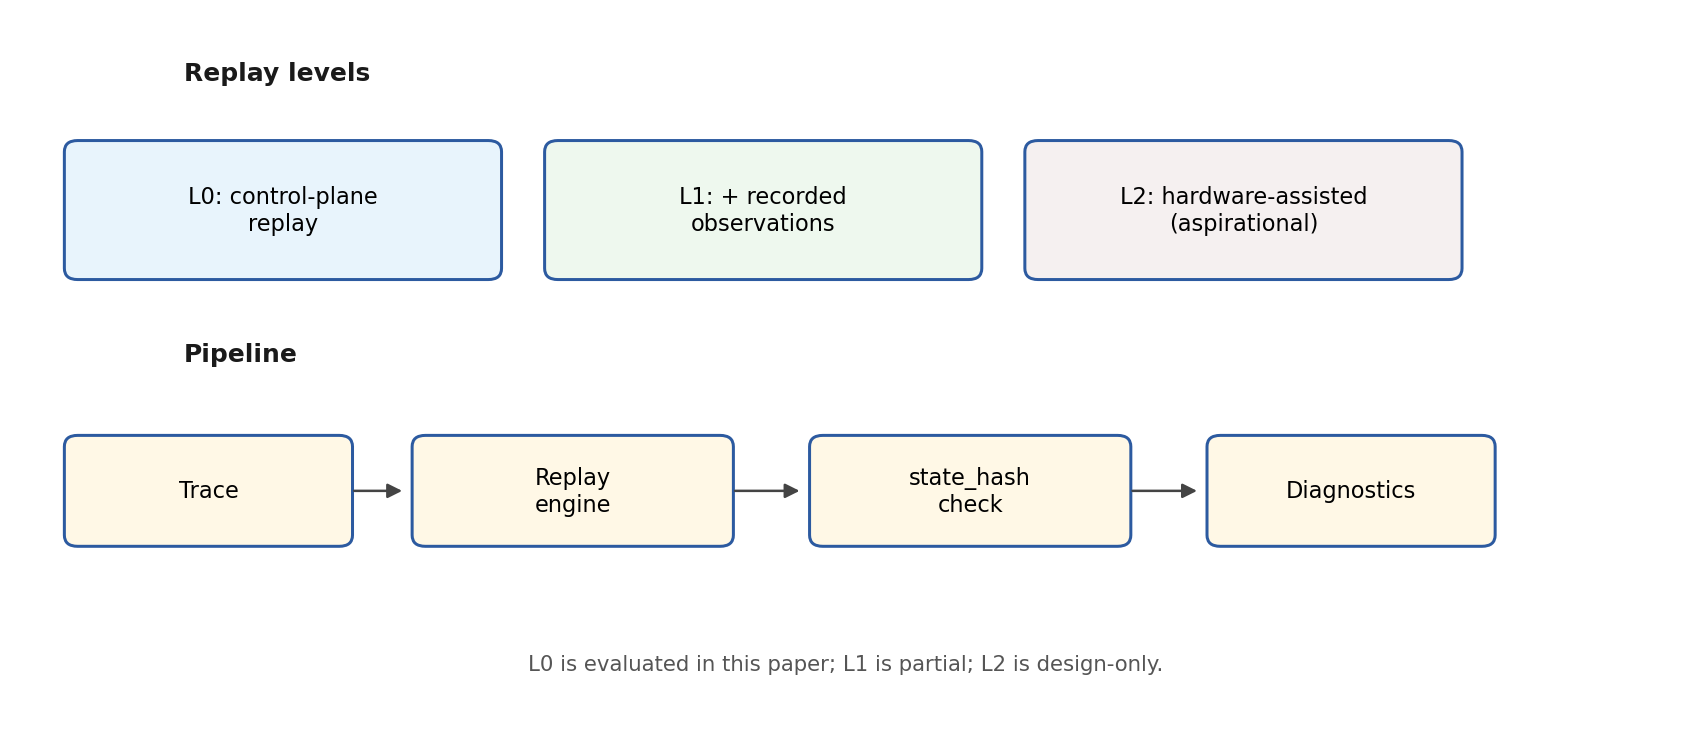
\includegraphics[width=0.92\linewidth]{figures/p3_replay_levels_diagram.png}
}{
    \fbox{\parbox[c][5cm][c]{0.92\linewidth}{\centering Placeholder for Figure 0: replay levels and replay pipeline.\\Source: \tool{export\_p3\_replay\_levels\_figure.py}.}}
}
\caption{Replay levels and replay pipeline. \Lzero{} is implemented and evaluated; \Lone{} is a partial control-plane twin contract; \Ltwo{} is design-only in this version.}
\label{fig:levels}
\end{figure}

\subsection{Replay engine}

The replay engine takes a trace conforming to the schema, re-applies events in sequence order, recomputes control-plane state, and checks each committed state hash. The default implementation corresponds to \Lzero{} replay.

The evaluated engine exposes three timing-relevant modes:

\begin{itemize}[leftmargin=1.5em]
    \item \textbf{apply-only, no hash.} Events are applied but no verification is performed. This is the lower-bound baseline.
    \item \textbf{final-hash-only.} Only the final state hash is checked. This gives some verification power but no per-event localization.
    \item \textbf{full \Lzero{}.} Per-event state-hash checks and structured diagnostics are enabled.
\end{itemize}

These baselines matter because the main replay question is not just “does the tool work?” but “what does structured verification cost relative to weaker alternatives?”

\subsection{Diagnostics and witness slices}

When replay diverges, the system emits structured diagnostics that include:
\begin{itemize}[leftmargin=1.5em]
    \item \field{divergence\_at\_seq},
    \item \field{expected\_hash},
    \item \field{got\_hash},
    \item event type and actor context,
    \item a witness slice used to support forensic localization.
\end{itemize}

The goal is not simply to mark a trace as failed, but to make the failure admissible as evidence and useful for audit or reconstruction.

\subsection{\Lone{} twin contract}

The artifact includes an \Lone{} stub and an optional \tool{--l1-twin} path. In this paper, \Lone{} means \Lzero{} plus deterministic twin replay over recorded observations and declared twin identity parameters such as build hash, model parameters, and environment seed. It does \emph{not} mean physics replay. We state this explicitly because “twin replay” is otherwise easy to over-interpret.

\subsection{Evidence integration}

Replay outcomes are written into an evidence bundle through fields such as \field{replay\_ok} and \field{replay\_diagnostics}. The concrete schema is versioned as \code{kernel/mads/EVIDENCE\_BUNDLE.v0.1.schema.json}; the portfolio maps trace-level replay results into bundle-shaped records in \code{impl/src/labtrust\_portfolio/evidence.py}. This is not a cosmetic integration. It is part of the motivation for the design: replay becomes admissible evidence inside a broader assurance workflow rather than remaining a developer-only debugging artifact.
For example, if replay diverges at \field{seq=7}, the diagnostic object records expected hash, observed hash, event context, and witness slice; the bundle records \field{replay\_ok=false} and a concise diagnostic summary. An auditor can then validate the artifact path independently without re-running an opaque internal pipeline.

\section{Methodology}

\subsection{Corpus}

The replay corpus is discovered from trace/expected-output pairs under the replay benchmark directory. Results are reported using explicit evidence lanes (\field{corpus\_category}): synthetic traps, synthetic passes, field-proxy traces, and real-ingest traces.

\begin{enumerate}[leftmargin=1.5em]
    \item \textbf{Synthetic pass traces.} Thin-slice and benign passes used for overhead and fidelity checks.
    \item \textbf{Synthetic trap traces.} Controlled failures including nondeterminism, reorder, timestamp-order mismatch, hash mismatch, long-horizon mismatch, and mixed-failure traces.
    \item \textbf{Field-proxy traces.} TRACE-conformant synthetic traces such as \code{field\_style\_pass} used as an external-validity proxy for mapped logs.
    \item \textbf{Real-ingest lane.} A redacted/template real-ingest example such as \code{real\_bucket\_example} kept visible as a distinct evidence lane.
\end{enumerate}

The trap corpus is especially important because it makes localization measurable. The evaluation does not merely ask whether replay passes or fails; it checks whether the first divergence is reported at the expected sequence.

\subsection{Metrics}

We use four classes of metrics.

\paragraph{Replay fidelity.}
For each corpus trace, replay should either pass or fail according to the expected outcome. For failing trap traces, the divergence sequence should match the expected sequence.

\paragraph{Localization quality.}
The summary reports a localization-confidence-style metric over sequence-expected traps, binomial Wilson 95\% intervals for corpus-level rates (\field{divergence\_localization\_wilson\_ci95}, \field{corpus\_outcome\_wilson\_ci95}), and records whether all expected outcomes were met.

\paragraph{Overhead.}
For the primary thin-slice trace, we measure replay time over repeated runs and report empirical mean, standard deviation, p95, and p99 using linear Hyndman--Fan type-7 percentiles \cite{hyndman1996quantiles}. Bootstrap confidence intervals are supported by the evaluation script for the publishable run.

\paragraph{Baseline cost.}
We compare full \Lzero{} replay against apply-only and final-hash-only baselines to quantify the incremental cost of structured verification and localization.

\subsection{Run configuration}

The minimal run uses fewer repetitions and bootstrap draws. The publishable configuration uses:
\begin{itemize}[leftmargin=1.5em]
    \item \tool{--overhead-runs 20},
    \item \tool{--thin-slice-seeds 42,43,44,45,46},
    \item \tool{--bootstrap-reps 500},
    \item optional \tool{--overhead-curve}.
\end{itemize}

The summary JSON records the run manifest, platform, Python version, trace corpus, percentile method, and overhead settings. This is important because overhead results are microbenchmark-sensitive and should not be reported without manifest context.

\subsection{Protocol and failure criteria}
The publishable protocol binds claims to one manifest: \field{overhead\_runs=20}, \field{thin\_slice\_seeds=42,43,44,45,46}, \field{bootstrap\_reps>=500}, and schema version \field{p3\_replay\_eval\_v0.2}. A corpus row is counted as failure if observed replay outcome or expected divergence sequence disagrees with the expected file. For denominator hygiene, \code{thin\_slice} is included in corpus row totals but excluded from trap-only localization denominators. Wilson bounds are reported for transparency on small sample sizes and should be interpreted as conservative uncertainty envelopes, not tight asymptotic estimates.

\section{Results}

\subsection{Corpus outcomes and localization}

Question: does the replay contract behave correctly on the corpus?  
Answer: yes. The summary records \field{corpus\_expected\_outcomes\_met=true}; pass traces replay successfully and seq-labeled trap traces diverge at the expected sequence.  
Why it matters: this is the core assurance claim, namely that \Lzero{} replay provides independently checkable control-plane evidence and first-divergence localization under declared semantics.
Claim link: this subsection provides primary evidence for C1 and for C2's localization component.

Table~\ref{tab:corpus} summarizes the corpus lanes and localization-relevant fields. The artifact includes a fully generated per-trace table in \code{generated\_tables.md}; the table here is a compact paper-facing synthesis.

\begin{table}[H]
\centering
\caption{Replay corpus summary by evidence lane, showing which rows are eligible for seq-level localization and which rows provide pass/fail-only evidence.}
\label{tab:corpus}
\begin{tabular}{p{2.8cm}p{3.2cm}p{1.1cm}p{1.4cm}p{1.5cm}p{2.6cm}}
\toprule
Lane / family & Representative rows & Count & Seq-localizable? & Localization correct? & Role in evaluation \\
\midrule
Synthetic pass & thin\_slice, benign\_perturbation\_pass & 2 & no & n/a & Fidelity and overhead anchor \\
Field proxy & field\_style\_pass, field\_style\_pass\_variant\_b & 2 & no & n/a & External-validity proxy lane \\
Real ingest & real\_bucket\_example & 1 & no & n/a & Real-trace lane visibility \\
Synthetic trap & nondeterminism, reorder, timestamp\_reorder, hash\_mismatch, long\_horizon, mixed\_failure & 6 & yes & yes (6/6) & Localization stress and diagnostics \\
\bottomrule
\end{tabular}
\end{table}

Localization denominator clarity is explicit in the run: total corpus rows = 11 including thin-slice; seq-localizable rows = 6; pass/fail-only rows = 5. This prevents conflating lane coverage with localization confidence.

The evaluator also reports binomial Wilson 95\% confidence intervals for corpus-level rates (small corpus: interpret as conservative bounds, not tight estimation): \field{divergence\_localization\_wilson\_ci95} $= [0.6097,\,1.0]$ for localization correctness on seq-labeled traps and \field{corpus\_outcome\_wilson\_ci95} $= [0.7225,\,1.0]$ for per-trace expected outcomes, on the evaluated publishable run.

\begin{table}[H]
\centering
\caption{Per-trace localization and corpus space extension (paired with the lane summary table). Columns report localization match/ambiguity, inferred mismatch family, on-disk trace footprint, and diagnostic payload size.}
\label{tab:corpus-1b}
\resizebox{\textwidth}{!}{%
\begin{tabular}{lccccccc}
\toprule
Trace & \field{corpus\_category} & loc.\ match & ambiguous & root cause & bytes & hash fields & diag.\ bytes \\
\midrule
thin\_slice & synthetic\_pass & true & false & --- & 3388 & 12 & --- \\
benign\_perturbation\_pass & synthetic\_pass & true & false & --- & 1901 & 5 & --- \\
field\_style\_pass & field\_proxy & true & false & --- & 4932 & 12 & --- \\
field\_style\_pass\_variant\_b & field\_proxy & true & false & --- & 2408 & 6 & --- \\
hash\_mismatch\_trap & synthetic\_trap & true & false & tool\_io & 1061 & 3 & 850 \\
long\_horizon\_trap & synthetic\_trap & true & false & tool\_io & 7233 & 21 & 869 \\
mixed\_failure\_trap & synthetic\_trap & true & false & tool\_io & 2263 & 6 & 1285 \\
nondeterminism\_trap & synthetic\_trap & true & false & tool\_io & 519 & 1 & 452 \\
real\_bucket\_example & real\_ingest & true & false & --- & 1319 & 3 & --- \\
reorder\_trap & synthetic\_trap & true & false & tool\_io & 784 & 2 & 651 \\
timestamp\_reorder\_trap & synthetic\_trap & true & false & tool\_io & 804 & 2 & 651 \\
\bottomrule
\end{tabular}%
}
\end{table}

\begin{figure}[H]
\centering
\IfFileExists{figures/p3_corpus_lane_counts.png}{
    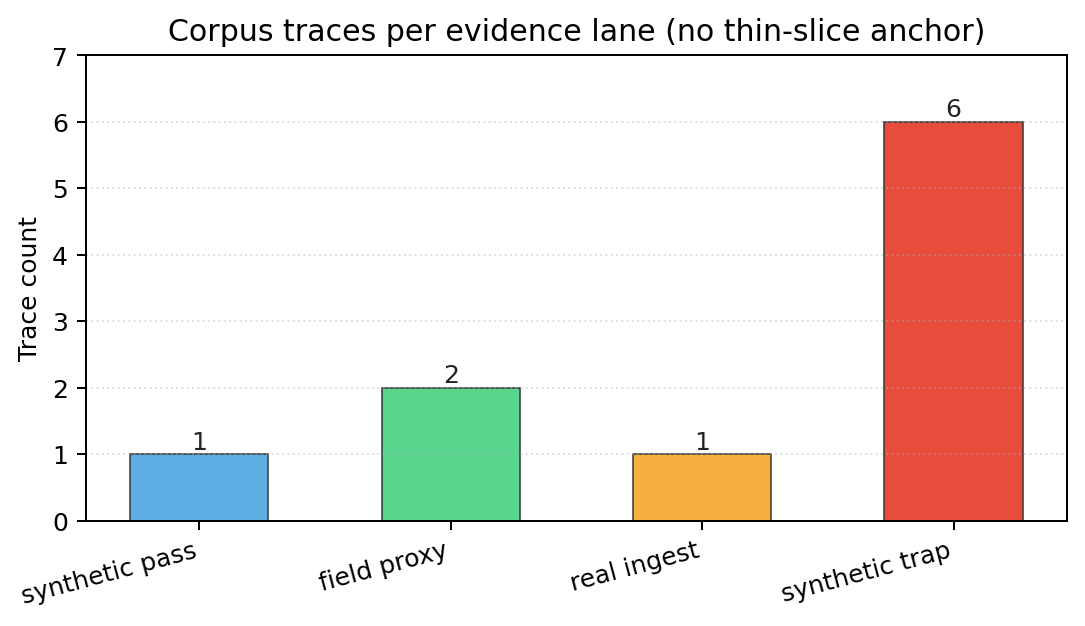
\includegraphics[width=0.62\linewidth]{figures/p3_corpus_lane_counts.png}
}{
    \fbox{\parbox[c][3.5cm][c]{0.62\linewidth}{\centering Placeholder: corpus traces per evidence lane.\\Source: \tool{plot\_p3\_corpus\_lanes.py}.}}
}
\caption{Corpus trace count by evidence lane (excluding the thin-slice overhead anchor).}
\label{fig:corpus-lanes}
\end{figure}

\begin{table}[H]
\centering
\caption{Failure-diversity summary for the synthetic-trap lane.}
\label{tab:failure-diversity}
\begin{tabular}{p{4.2cm}cc}
\toprule
Mismatch family & Rows & First-divergence seq (expected) \\
\midrule
Immediate mismatch & 1 & 0 \\
Reorder mismatch & 1 & 1 \\
Timestamp-order mismatch & 1 & 1 \\
Explicit hash mismatch & 1 & 1 \\
Long-horizon mismatch & 1 & 20 \\
Mixed-failure trace & 1 & 2 \\
\bottomrule
\end{tabular}
\end{table}

\subsection{Full \Lzero{} overhead}

Question: what is the cost of full per-event verification on the primary thin-slice workload?  
Answer: full \Lzero{} replay remains sub-millisecond at publishable settings.  
Why it matters: bounded verification overhead makes replay usable as routine assurance infrastructure instead of a rare forensic-only path.
Claim link: this subsection supports the cost component of C2 and the deployability component of C1.

\begin{table}[H]
\centering
\caption{Full \Lzero{} replay overhead on the primary thin-slice trace (seed 42) over 20 replay runs; percentiles use empirical Hyndman--Fan type-7 estimates.}
\label{tab:l0-overhead}
\begin{tabular}{ccccc}
\toprule
$n_{\text{replays}}$ & mean (ms) & stdev (ms) & p95 (ms) & p99 (ms) \\
\midrule
20 & 0.3495 & 0.1680 & 0.6911 & 0.7821 \\
\bottomrule
\end{tabular}
\end{table}

For the intended use case --- control-plane audit and evidence generation --- these numbers are operationally small. They do not imply fleet-scale cost, distributed ingest cost, or large-trace throughput, but they do support bounded verification overhead on the evaluated thin-slice workload.

\subsection{Baselines and incremental verification cost}

Question: what does structured verification add versus weaker alternatives?  
Answer: full \Lzero{} is measurably slower than apply-only and final-hash-only, with paired full-vs-apply-only difference mean 0.3251\,ms (95\% bootstrap CI [0.2613, 0.3989]).  
Why it matters: this quantifies the price of admissible evidence (per-event commitments and witness diagnostics), not merely replay speed.
Claim link: this subsection is direct evidence for C2.

\begin{table}[H]
\centering
\caption{Baseline comparison on the same primary thin-slice trace: apply-only is the lower bound, final-hash-only verifies only terminal state, and full \Lzero{} adds per-event localization.}
\label{tab:baselines}
\begin{tabular}{lccp{5.0cm}}
\toprule
Variant & mean time (ms) & Approx.\ added cost vs apply-only (ms) & Interpretation \\
\midrule
Apply-only, no hash & 0.0244 & 0.0000 & Lower bound; no verification, no audit \\
Final-hash-only & 0.0783 & 0.0539 & End-state verification only; no per-event localization \\
Full \Lzero{} replay & 0.3495 & 0.3251 & Per-event checks and structured diagnostics \\
\bottomrule
\end{tabular}
\end{table}

\begin{figure}[H]
\centering
\IfFileExists{figures/p3_baseline_mean_ms.png}{
    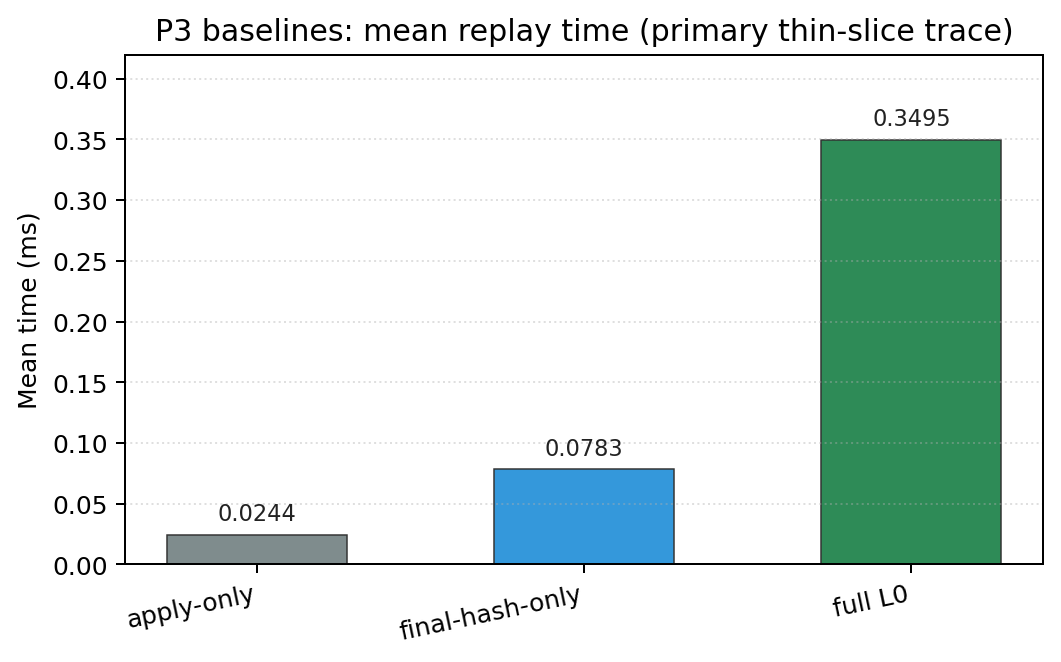
\includegraphics[width=0.72\linewidth]{figures/p3_baseline_mean_ms.png}
}{
    \fbox{\parbox[c][4cm][c]{0.72\linewidth}{\centering Placeholder for baseline mean replay time by mode.\\Source: \tool{plot\_p3\_baseline\_bars.py}.}}
}
\caption{Mean replay time (ms) for apply-only, final-hash-only, and full \Lzero{} on the primary thin-slice trace (same run as Table~\ref{tab:baselines}).}
\label{fig:baseline-bars}
\end{figure}

The baseline story is central to the paper. If one only cared about re-applying events, replay would be cheap but evidentially weak. The extra cost is exactly what buys localizable divergence detection.

\subsection{Overhead curve and multi-seed family}

Question: are results robust across event-prefix sizes and multiple seeds?  
Answer: the artifact reports overhead curve points for trace prefixes and a five-seed thin-slice family with across-seed variability in \field{multi\_seed\_overhead}; on the current publishable run, the across-seed mean of means is 0.2990\,ms with across-seed stdev 0.0765\,ms.  
Why it matters: this reduces single-seed overfitting risk while remaining transparent about small-trace, in-process scope.

\begin{figure}[H]
\centering
\IfFileExists{figures/p3_replay_overhead.png}{
    
\includegraphics[width=0.78\linewidth]{figures/p3_replay_overhead.png}
}{
    \fbox{\parbox[c][5cm][c]{0.78\linewidth}{\centering Placeholder for replay overhead versus trace size.\\Source: \tool{plot\_replay\_overhead.py}.}}
}
\caption{Replay overhead versus trace size for prefixes of the primary thin-slice trace; bootstrap confidence intervals appear as error bars when available.}
\label{fig:overhead}
\end{figure}

\subsection{First-divergence localization visual}

Figure~\ref{fig:first-divergence} instantiates the localization story on a representative trap trace (\code{mixed\_failure\_trap}) from the evaluated corpus: committed versus replayed hashes by event index, first divergence highlighted, witness slice centered on the divergence, and downstream events de-emphasized as unnecessary to establish first contract violation. The figure is generated from the current replay artifact via \tool{export\_p3\_first\_divergence\_timeline.py}.
Claim link: this subsection visually supports C1 and C3.

\begin{figure}[H]
\centering
\IfFileExists{figures/p3_first_divergence_timeline.png}{
    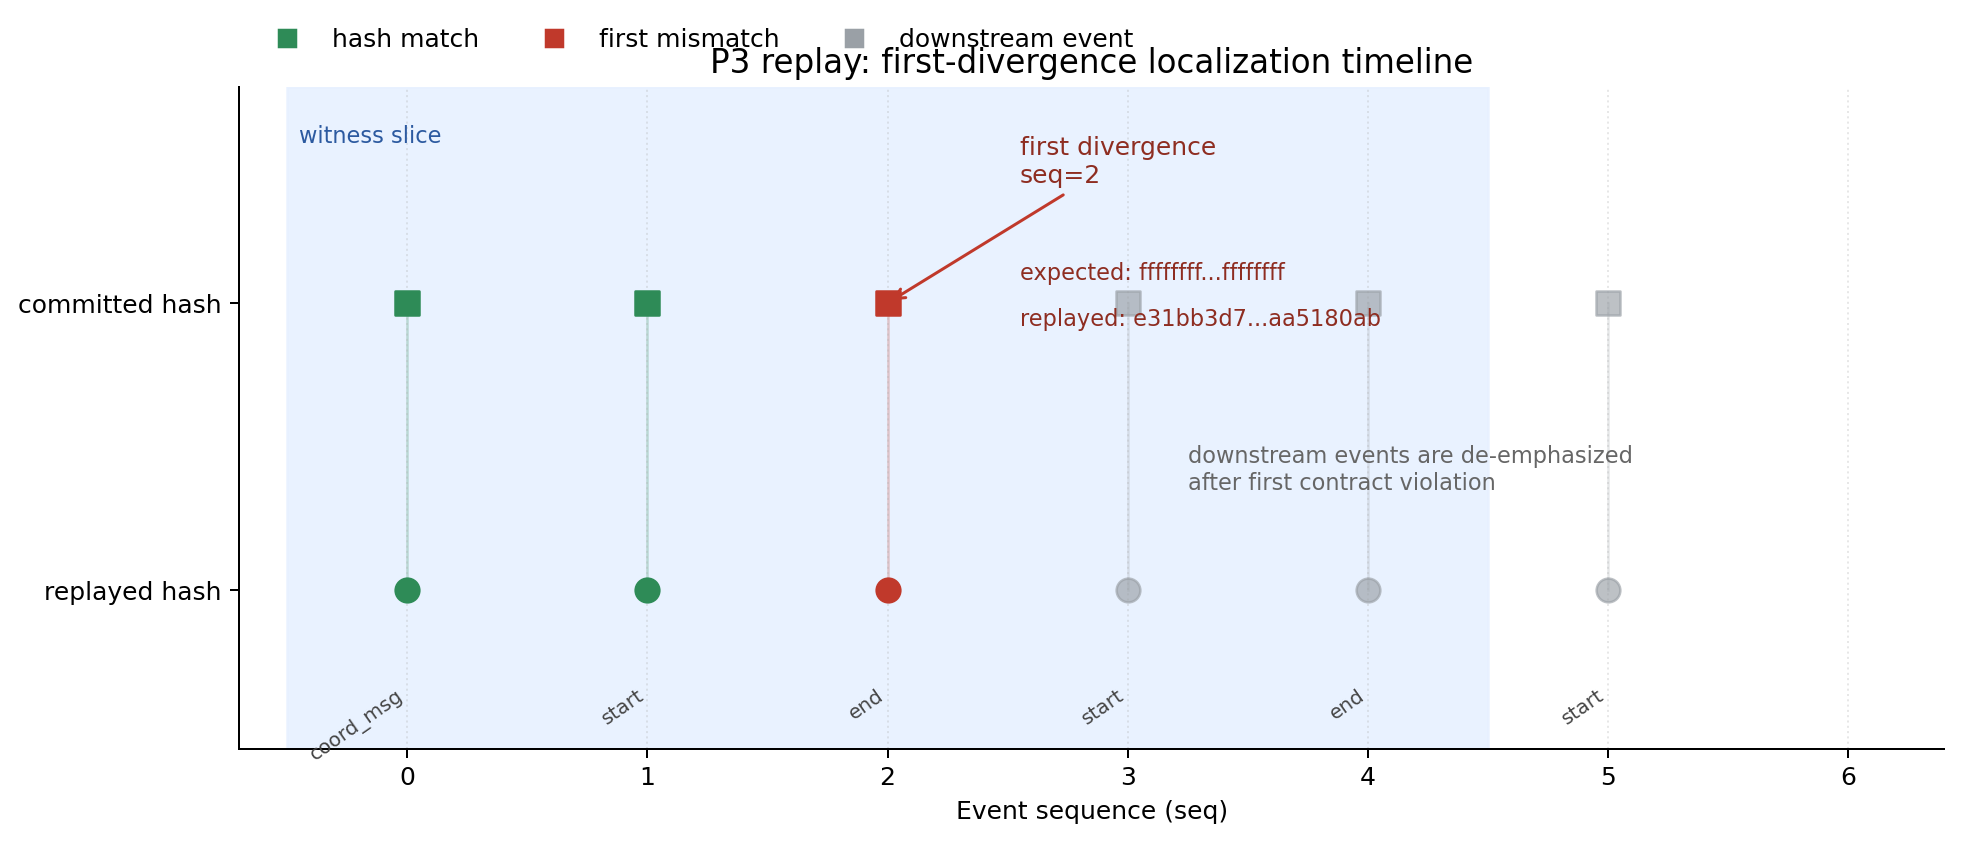
\includegraphics[width=0.88\linewidth]{figures/p3_first_divergence_timeline.png}
}{
    \fbox{\parbox[c][5cm][c]{0.88\linewidth}{\centering Placeholder for first-divergence timeline visual.\\Spec: \code{papers/P3\_Replay/LOCALIZATION\_FIGURE\_SPEC.md}}}
}
\caption{First-divergence localization timeline: committed versus replayed state hashes by event sequence for a representative trap trace. Replay localizes the first contract violation at the highlighted sequence, shows witness context around that point, and de-emphasizes downstream events as unnecessary to establish the first violation.}
\label{fig:first-divergence}
\end{figure}

\subsection{\Lone{} status}

Question: what evidence is available for \Lone{} in this version?  
Answer: beyond \field{l1\_stub\_ok}, the artifact includes \field{l1\_twin\_summary} over five seeds (\field{all\_pass=true}, mean 1.7425\,ms, stdev 0.8187\,ms, min 1.0233\,ms, max 3.0904\,ms).  
Why it matters: this keeps \Lone{} secondary while demonstrating a concrete, measured extension path. The higher wall-clock time versus \Lzero{} on the thin slice is expected: the twin path exercises additional configuration and observation checks; it is not a claim that \Lone{} improves raw \Lzero{} throughput.
Claim link: this subsection provides supporting evidence for C3 (extension path), not the primary C1/C2 claim.

\begin{table}[H]
\centering
\caption{L1 twin supplementary summary from \field{l1\_twin\_summary}.}
\label{tab:l1-supp}
\begin{tabular}{lcccc}
\toprule
$n_{seeds}$ & all-pass & mean time (ms) & stdev (ms) & min/max (ms) \\
\midrule
5 & true & 1.7425 & 0.8187 & 1.0233 / 3.0904 \\
\bottomrule
\end{tabular}
\end{table}

\paragraph{Key takeaways.}
\begin{itemize}[leftmargin=1.5em]
    \item \textbf{C1}: lane-separated corpus outcomes and per-trace diagnostics show contract-bounded replay is operational as assurance evidence.
    \item \textbf{C2}: bounded overhead and baseline deltas quantify the measurable price of admissible replay verification.
    \item \textbf{C3/C4}: witness-oriented diagnostics and bundle mapping keep replay outputs directly usable for audit workflows.
\end{itemize}

\section{Discussion}

The main intellectual point is that replay in CPS should be treated as a \emph{contract-bounded evidentiary mechanism}, not merely as a debugging convenience. Three design choices follow from that view.

First, trace semantics must be explicit enough to support third-party verification. This is why we carry sequence numbers, structured payloads, and per-event state commitments. Second, replay claims must be tiered. A control-plane replay contract is useful, but it should not be mislabeled as full determinism. Third, diagnostics must be localizable. In safety and audit settings, “final state mismatch” is weaker than “the first divergence occurred at event 17 with this expected/observed state commitment pair.”

The baseline comparison also highlights something easy to miss: the dominant cost in this design is not replaying the trace, but making replay \emph{admissible}. Apply-only is extremely cheap. The extra cost of full \Lzero{} buys per-event verification and structured forensics. That is the relevant tradeoff for a systems paper in this niche.

\begin{table}[H]
\centering
\caption{Trace-to-evidence mapping for assurance use.}
\label{tab:evidence-map}
\begin{tabular}{p{2.7cm}p{3.4cm}p{3.4cm}p{3.2cm}}
\toprule
Trace field & Replay output & Evidence bundle field & Assurance use \\
\midrule
\field{events[].state\_hash\_after} & expected-vs-observed mismatch at seq $i^\star$ & \field{verification.replay\_diagnostics} & Localized forensic cause and audit trail \\
\field{events[].seq} & \field{divergence\_at\_seq} + witness context & \field{verification.replay\_ok} (false on divergence) & Explicit contract-failure index for reviewers \\
\field{final\_state\_hash} & final consistency check & \field{verification.replay\_ok} (true on full match) & Binary conformance claim for release gating \\
\bottomrule
\end{tabular}
\end{table}

The deployment path is straightforward in the intended setting: a controller emits TRACE-conformant events, nightly replay validation runs over completed workflows, failed replays generate evidence-bundle exceptions, and operators inspect witness slices for triage and remediation.

\section{Limitations and threats to validity}

\paragraph{Internal validity.}
Replay findings assume the replay engine implementation and transition semantics are correctly implemented for the declared control-plane contract. We mitigate this with corpus traps, deterministic checks, and strict summary verification, but implementation defects remain a standard threat in any replay system.

\paragraph{Construct validity.}
The primary construct is control-plane replay conformance, not full behavioral equivalence of physical systems. Hash equality is interpreted within the declared semantics and practical collision assumptions. This is intentional but narrower than equivalence over all latent system state.

\paragraph{External validity.}
The corpus includes synthetic traps, synthetic passes, field-proxy traces, and a real-ingest example. This supports mechanism evaluation and lane separation, but does not by itself establish production-fleet generalization. Field-proxy and real-ingest lanes depend on mapping external logs into the declared event ontology; ambiguous or lossy mapping can yield false replay failures or mask true divergence even when the replay engine is correct. Scaling real traces requires ingest discipline and schema alignment, not only more data volume.

\paragraph{Systems cost scope.}
Reported overhead is in-process replay cost on thin-slice workloads. It does not include log transport, distributed ingestion, storage backends, or deployment orchestration overhead.

\paragraph{Level scope.}
\Lone{} is partial in this version (control-plane twin replay over recorded observations), and \Ltwo{} is design-only. We do not claim full-process determinism, hardware equivalence, or physics replay.

\paragraph{Explicit non-goal / negative case.}
If traces omit per-event commitments or external logs are mapped ambiguously into the declared event semantics, replay may be unable to provide seq-level localization even when the implementation is correct. In such cases replay fails because the contract is intentionally narrower than the underlying system behavior, not because the checker is weak.

\paragraph{Threat model (assumptions).}
We assume a trusted replay engine and transition semantics for the declared \Lzero{} contract; an adversary who can alter the engine or the verifier can trivially falsify outcomes. Hash commitments are assumed collision-resistant for the evaluated traces. We do not assume tamper-evidence of the trace bytes at ingest; integrity and provenance of stored traces are orthogonal (e.g., append-only storage or signed artifacts) and are out of scope for this paper.

\section{Conclusion}

This paper presents a replay framework for agentic CPS built around replay levels and a concrete \Lzero{} contract. The central contribution is not full record/replay, but a reusable assurance mechanism: sequence-level detection and localization of control-plane divergence relative to declared trace semantics, exported as independently checkable evidence artifacts. The evaluated artifact combines a CPS-aware trace format, replay engine, structured diagnostics, explicit baselines, lane-separated corpus reporting, and evidence-bundle integration. On the evaluated corpus, expected outcomes are met and seq-labeled trap divergences localize at the expected event. On the primary thin-slice trace, full \Lzero{} replay remains sub-millisecond, with 0.3495\,ms mean overhead and empirical p99 below 1\,ms. This is sufficient to make replay practical as routine control-plane assurance infrastructure while remaining explicit about open scope: hardware determinism, physics replay, and production-scale deployment.

\appendix

\section{Reproducibility}

The evaluation is driven by \tool{scripts/replay\_eval.py}, which writes a structured summary JSON containing schema version, run manifest, percentile method, overhead statistics, corpus outcomes, baseline timings, and optional overhead-curve data. A publishable run uses:
\begin{quote}
\small
\tool{PYTHONPATH=impl/src python scripts/replay\_eval.py --out datasets/runs/replay\_eval/summary.json --overhead-curve --overhead-runs 20 --thin-slice-seeds 42,43,44,45,46 --bootstrap-reps 500 --l1-twin}
\end{quote}

The main post-processing scripts are:
\begin{itemize}[leftmargin=1.5em]
    \item \tool{scripts/export\_replay\_corpus\_table.py}
    \item \tool{scripts/export\_p3\_paper\_figures.py} (camera-ready PNGs under \code{papers/P3\_Replay/figures/}, including levels diagram, overhead curve, baselines, corpus lanes, first-divergence timeline)
    \item \tool{scripts/verify\_p3\_replay\_summary.py --strict-curve}
\end{itemize}

\section{Pre-submission checklist}
\begin{itemize}[leftmargin=1.5em]
    \item Numeric consistency verified across abstract, Tables~\ref{tab:l0-overhead}/\ref{tab:baselines}, and conclusion.
    \item Figure assets resolve from \code{papers/P3\_Replay/figures/} with no placeholder fallback.
    \item Claim map (Table~\ref{tab:claim-map}) references only tables/figures present in this draft.
    \item Repro command path regenerates summary, tables, and paper-facing figures from scripts.
    \item Bounded-scope language remains consistent (control-plane evidence, not full-process or physics replay).
\end{itemize}

\section{Claim-to-evidence map}

\begin{table}[H]
\centering
\caption{Claim-to-evidence map linking each paper claim to concrete tables, figures, and artifact paths.}
\label{tab:claim-map}
\begin{tabular}{p{1.2cm}p{9.5cm}p{3.1cm}}
\toprule
Claim & Statement & Primary evidence \\
\midrule
C1 & A CPS-aware trace format plus a determinism contract enables \Lzero{} replay with per-event verification and sequence-level localization of divergence across explicit evidence lanes. & Tables~\ref{tab:corpus}, \ref{tab:corpus-1b}, \ref{tab:failure-diversity}, \ref{tab:baselines}; Figures~\ref{fig:levels}, \ref{fig:corpus-lanes}, \ref{fig:first-divergence}, \ref{fig:overhead} \\
C2 & Hidden nondeterminism is detectable and localizable at first divergence, and baselines quantify the incremental cost of full verification. & Tables~\ref{tab:corpus}, \ref{tab:corpus-1b}, \ref{tab:l0-overhead}, \ref{tab:baselines}; Figure~\ref{fig:baseline-bars} \\
C3 & Replay supports audit-style reconstruction via witness slices and structured diagnostics, including an L1 extension path. & Tables~\ref{tab:corpus}, \ref{tab:l1-supp}, \ref{tab:evidence-map}; Figure~\ref{fig:first-divergence} \\
C4 & Replay outcomes integrate with evidence bundles as admissible machine-checkable assurance artifacts. & System design/evidence integration; Table~\ref{tab:evidence-map} \\
\bottomrule
\end{tabular}
\end{table}

\section{Why this is not a whole-process replay paper}

For clarity, Table~\ref{tab:related-systems} situates the paper's replay contract against stronger replay systems.

\begin{table}[H]
\centering
\caption{Positioning against stronger record/replay systems.}
\label{tab:related-systems}
\begin{tabular}{p{3.0cm}p{3.2cm}p{3.5cm}p{4.3cm}}
\toprule
System family & Primary guarantee & Typical scope & Why the present approach is preferable \\
\midrule
Whole-process record/replay (e.g., RR, ReVirt) & Replay of process or guest execution with stronger determinism assumptions & Process, syscalls, VM, or lower-level execution & When only control-plane evidence is needed and full-process determinism is infeasible or unnecessary \\
Secure-log accountability (e.g., PeerReview) & Fault detection and accountability via replay from secure logs & Distributed nodes and message histories & When the main goal is localizable control-plane replay integrated into a CPS evidence pipeline \\
Log-only tools & Observability of events & Events only & When audit requires detection of replay divergence, not just retained logs \\
This paper's \Lzero{} & Control-plane replay with per-event state-hash verification & CPS trace semantics and control-plane state & When sequence-level nondeterminism localization is required without overclaiming full determinism \\
\bottomrule
\end{tabular}
\end{table}

\begin{thebibliography}{9}

\bibitem{dunlap2002revirt}
George W. Dunlap, Samuel T. King, Sukru Cinar, Murtaza A. Basrai, and Peter M. Chen.
\newblock ReVirt: Enabling intrusion analysis through virtual-machine logging and replay.
\newblock In \emph{Proceedings of the 5th Symposium on Operating Systems Design and Implementation (OSDI)}, pages 211--224, 2002.

\bibitem{ocallahan2017rr}
Robert O'Callahan, Chris Jones, Nathan Froyd, Kyle Huey, Albert Noll, and Nimrod Partush.
\newblock Engineering record and replay for deployability.
\newblock In \emph{Proceedings of the 2017 USENIX Annual Technical Conference (USENIX ATC)}, pages 377--389, 2017.

\bibitem{haeberlen2007peerreview}
Andreas Haeberlen, Petr Kuznetsov, and Peter Druschel.
\newblock PeerReview: Practical accountability for distributed systems.
\newblock In \emph{Proceedings of the 21st ACM Symposium on Operating Systems Principles (SOSP)}, pages 175--188, 2007.

\bibitem{nist2017cps}
Edward A. Griffor, Chris Greer, David A. Wollman, and Martin Burns.
\newblock \emph{Framework for Cyber-Physical Systems: Volume 1, Overview}.
\newblock NIST Special Publication 1500--201, National Institute of Standards and Technology, 2017.

\bibitem{hyndman1996quantiles}
Rob J. Hyndman and Yanan Fan.
\newblock Sample quantiles in statistical packages.
\newblock \emph{The American Statistician}, 50(4):361--365, 1996.

\bibitem{w3c2013prov}
World Wide Web Consortium.
\newblock PROV-DM: The PROV data model.
\newblock W3C Recommendation, 2013.

\end{thebibliography}

\end{document}
